\documentclass[a4paper,10pt]{article}

% Packages
\usepackage[utf8]{inputenc}
\usepackage[T1]{fontenc}
\usepackage{amsmath}
\usepackage{txfonts}
\usepackage{titlesec}
\usepackage{geometry}
\usepackage{graphicx}
\usepackage{fancyhdr}
\usepackage{hyperref}
\usepackage{float}
\usepackage{caption}
\usepackage{booktabs}
\usepackage{array}
\usepackage[version=4]{mhchem}
\usepackage{siunitx}

\sisetup{per-mode=symbol, output-decimal-marker={,}}

% MISE EN PAGE
\geometry{a4paper, top=20mm, bottom=20mm, left=20mm, right=20mm}
\setlength{\parindent}{0pt}
\setlength{\parskip}{4pt}

\titleformat{\section}
  {\normalfont\bfseries\large}{\thesection.}{0.5em}{}[\titlerule]
\titleformat{\subsection}
  {\normalfont\bfseries}{\thesubsection.}{0.5em}{}

% En-tete / pied de page
\pagestyle{fancy}
\fancyhf{}
\lhead{\small Chimie Organique --- Travail Obligatoire}
\rhead{\small MT\_244 Semestre 2 --- 2025/2026}
\cfoot{\thepage}
\renewcommand{\headrulewidth}{0.4pt}

\hypersetup{colorlinks=true, linkcolor=black, urlcolor=blue, citecolor=black}

\newcommand{\og}{\guillemotleft\,}
\newcommand{\fg}{\,\guillemotright}

\begin{document}

% TITRE
\begin{center}
  {\LARGE \textbf{Travail Obligatoire --- Chimie Organique}}\\[6pt]
  {\large MT\_244 --- Semestre 2 --- 2025/2026}\\[4pt]
  {\normalsize Fili\`{e}re Microtechnique --- HEPIA, HES-SO Gen\`{e}ve}\\[6pt]
  \rule{\linewidth}{0.8pt}\\[4pt]
  {\large Guilhem Rozier}\\
  {\small \texttt{guilhem.roziervi@etu.hesge.ch}}\\[4pt]
  \rule{\linewidth}{0.4pt}
\end{center}

\vspace{4mm}

%======================================================================
\section{Solvant : Ac\'{e}tate d'\'{e}thyle}

\subsection{Formule semi-d\'{e}velopp\'{e}e}

\begin{figure}[H]
  \centering
  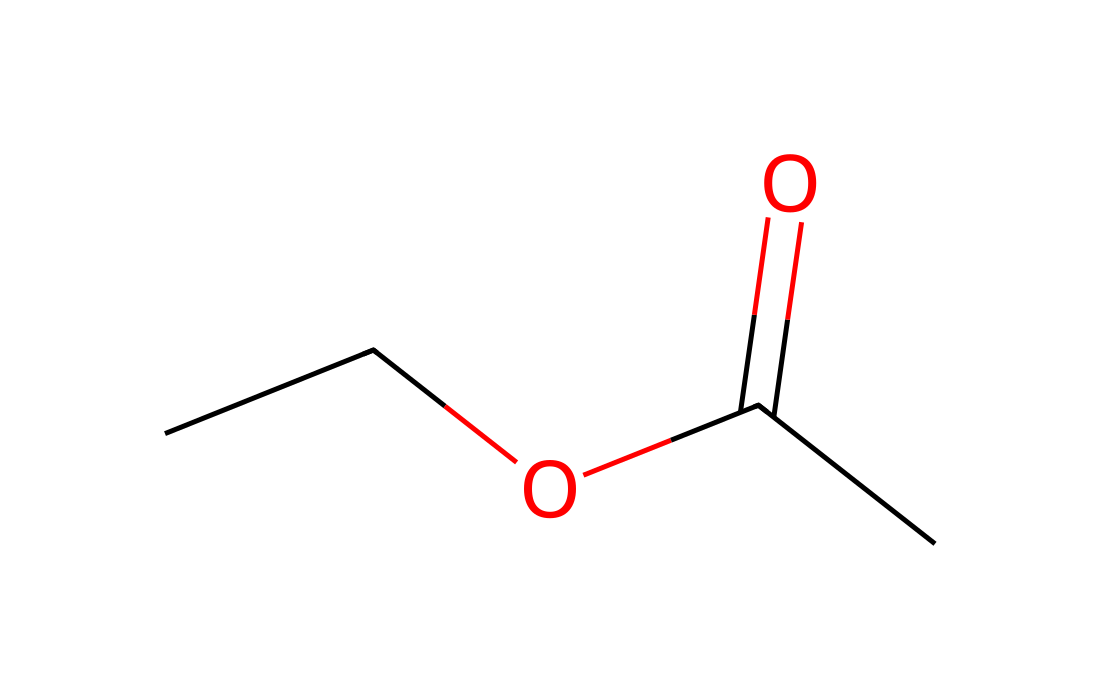
\includegraphics[width=0.45\linewidth]{Images/ethyl_acetate.png}
  \caption{Structure b\^{a}tonnets de l'ac\'{e}tate d'\'{e}thyle
    (\ce{CH3COOC2H5}), $M_M = \SI{88.11}{g/mol}$.}
  \label{fig:ea}
\end{figure}

\subsection{Type}
\begin{itemize}
  \item \textbf{Groupe fonctionnel :} ester (liaison \ce{-COO-})
  \item \textbf{Polarit\'{e} :} polaire aprotique (pas de H labile ; $\varepsilon_r \approx 6{,}0$)
\end{itemize}

\subsection{Donn\'{e}es physiques}

\begin{center}
\begin{tabular}{ll}
  \toprule
  Param\`{e}tre & Valeur \\
  \midrule
  Formule brute            & \ce{C4H8O2} \\
  Masse molaire            & \SI{88.11}{g/mol} \\
  Point de fusion          & \SI{-83.6}{\celsius} \\
  Point d'\'{e}bullition   & \SI{77.1}{\celsius} \\
  Densit\'{e} (\SI{20}{\celsius}) & \SI{0.902}{g/cm^3} \\
  Miscibilit\'{e} eau      & Partiellement miscible (\SI{8.3}{g/100mL} \`{a} \SI{20}{\celsius}) \\
  $\varepsilon_r$          & $\approx 6{,}0$ \\
  \bottomrule
\end{tabular}
\end{center}

\medskip
Liquide incolore \`{a} odeur fruiti\`{e}re caract\'{e}ristique. Partiellement miscible avec l'eau ;
miscible avec \'{e}thanol, ac\'{e}tone, di\'{e}thyl\'{e}ther.

\subsection{Inflammabilit\'{e} et toxicit\'{e}}
\begin{itemize}
  \item \textbf{H225} --- Liquide et vapeurs tr\`{e}s inflammables (point d'\'{e}clair : \SI{-4}{\celsius})
  \item \textbf{H319} --- Provoque une s\'{e}v\`{e}re irritation des yeux
  \item \textbf{H336} --- Peut provoquer somnolence ou vertiges
  \item \textbf{EUH066} --- Exposition r\'{e}p\'{e}t\'{e}e : dess\`{e}chement ou ger\c{c}ures de la peau
\end{itemize}
Faiblement toxique. En milieu acide ou basique, hydrolyse lente en \'{e}thanol et acide ac\'{e}tique.

\subsection{Utilisations}
\begin{itemize}
  \item Solvant de vernis, laques, peintures et adh\'{e}sifs
  \item Extraction analytique (chromatographie, HPLC)
  \item Parfumerie et ar\^{o}mes alimentaires (ar\^{o}me de poire/fraise)
  \item D\'{e}graissage industriel
  \item Recristallisation en synth\`{e}se organique
\end{itemize}

%======================================================================
\section{Polym\`{e}re : Polyt\'{e}trafluoro\'{e}thyl\`{e}ne (PTFE -- T\'{e}flon\textsuperscript{\textregistered})}

\subsection{Formule semi-d\'{e}velopp\'{e}e}

\begin{figure}[H]
  \centering
  \begin{minipage}{0.42\linewidth}
    \centering
    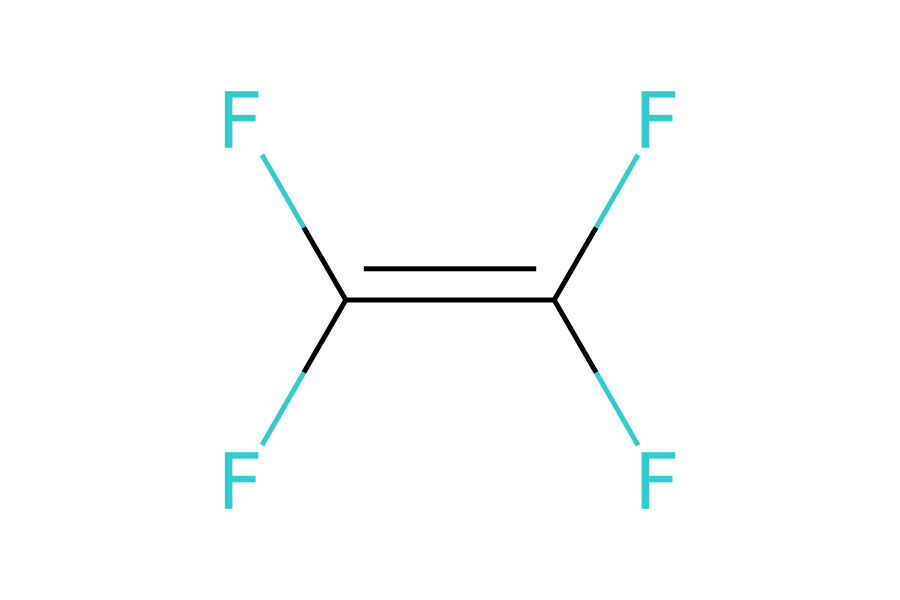
\includegraphics[width=\linewidth]{Images/TFE_monomer.png}
    \caption{Monom\`{e}re : t\'{e}trafluoro\'{e}thyl\`{e}ne (TFE, \ce{C2F4}).}
    \label{fig:tfe}
  \end{minipage}
  \hfill
  \begin{minipage}{0.42\linewidth}
    \centering
    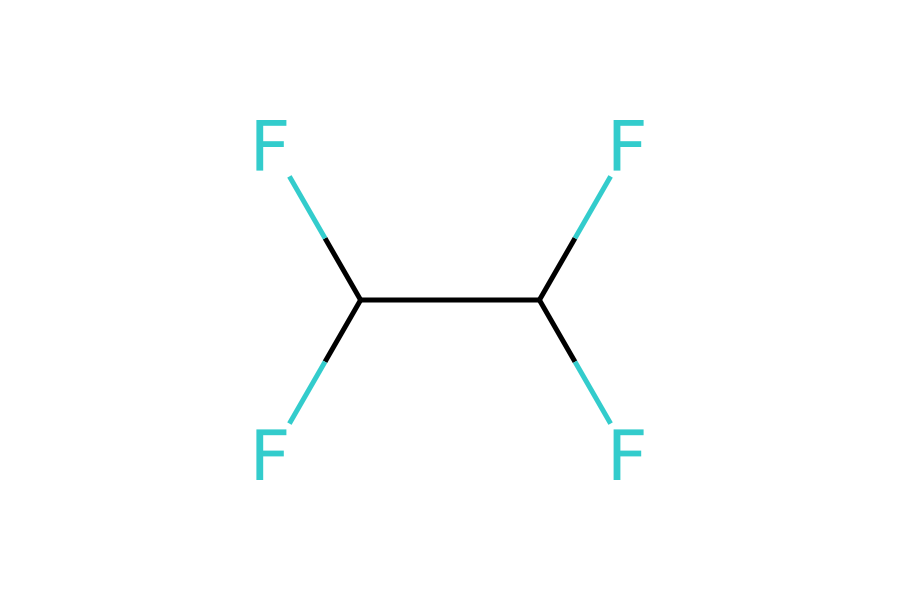
\includegraphics[width=\linewidth]{Images/PTFE_repeat.png}
    \caption{Unit\'{e} r\'{e}p\'{e}titive du PTFE : $-[\ce{CF2-CF2}]_n-$.}
    \label{fig:ptfe}
  \end{minipage}
\end{figure}

Unit\'{e} r\'{e}p\'{e}titive : $-[\ce{CF2-CF2}]_n-$,
avec $n \sim 10^5$--$10^6$, masses molaires de $10^6$--$10^7$~\si{g/mol}.

\subsection{Type}
\begin{itemize}
  \item \textbf{Groupe(s) fonctionnel(s) :} halog\'{e}n\'{e} fluor\'{e}
    (liaisons \ce{C-F} exclusivement sur la cha\^{\i}ne principale)
  \item \textbf{Comportement :} thermoplastique semi-cristallin
    ($T_f \approx \SI{327}{\celsius}$) ;
    viscosit\'{e} fondue extr\^{e}mement \'{e}lev\'{e}e --- mis en forme par frittage
\end{itemize}

\subsection{Propri\'{e}t\'{e}s remarquables}

\begin{center}
\begin{tabular}{ll}
  \toprule
  Propri\'{e}t\'{e} & Valeur / commentaire \\
  \midrule
  $T_f$                           & \SI{327}{\celsius} \\
  Utilisation continue max.       & \SI{260}{\celsius} \\
  Densit\'{e}                     & \SI{2.15}{}--\SI{2.20}{g/cm^3} \\
  Coefficient de frottement       & $0{,}04$--$0{,}10$ (parmi les plus faibles) \\
  R\'{e}sistance chimique         & Quasi-universelle (inerte acides, bases, solvants) \\
  \'{E}nergie de surface          & $\approx \SI{18}{mN/m}$ (non-mouillable) \\
  R\'{e}sistivit\'{e} \'{e}lectrique & $> 10^{18}\ \Omega\cdot\mathrm{cm}$ (isolant) \\
  \bottomrule
\end{tabular}
\end{center}

\medskip
L'inertie chimique exceptionnelle d\'{e}coule de la force des liaisons \ce{C-F}
(BDE $\approx \SI{544}{kJ/mol}$) et de l'\'{e}crantage total du squelette carbon\'{e}
par les atomes de fluor.

\subsection{Utilisations}
\begin{itemize}
  \item Rev\^{e}tements anti-adh\'{e}sifs (po\^{e}les, ustensiles de cuisine)
  \item Joints d'\'{e}tanch\'{e}it\'{e} industrie chimique et p\'{e}troli\`{e}re
  \item Isolation c\^{a}bles \'{e}lectriques haute performance
  \item Prot\`{e}ses vasculaires et implants m\'{e}dicaux (biocompatibilit\'{e})
  \item Membrane Gore-Tex\textsuperscript{\textregistered} (ePTFE)
  \item Plomberie : ruban d'\'{e}tanch\'{e}it\'{e} (\og ruban t\'{e}flon\fg)
\end{itemize}

%======================================================================
\section{Mol\'{e}cule pharmaceutique : Cannabidiol (CBD)}

\subsection{Formule semi-d\'{e}velopp\'{e}e}

\begin{figure}[H]
  \centering
  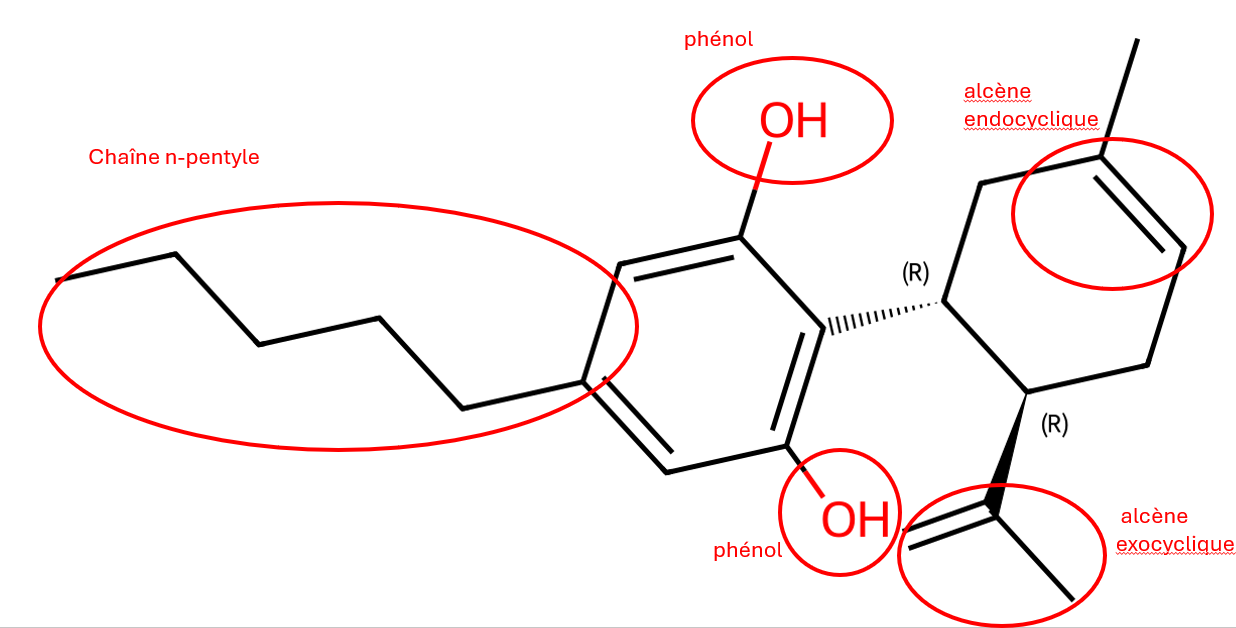
\includegraphics[width=0.65\linewidth]{Images/CBD.png}
  \caption{Structure b\^{a}tonnets du cannabidiol (CBD, \ce{C21H30O2}),
           $M_M = \SI{314.46}{g/mol}$.}
  \label{fig:cbd}
\end{figure}

\subsection{Groupes fonctionnels}

\begin{center}
\begin{tabular}{lll}
  \toprule
  Groupe fonctionnel & Formule & Localisation \\
  \midrule
  Ph\'{e}nol ($\times 2$)  & \ce{Ar-OH}           & Positions 1 et 3 du cycle aromatique \\
  Alc\`{e}ne endocyclique  & $>\mathrm{C{=}C}<$   & Double liaison dans le cyclohex\`{e}ne \\
  Alc\`{e}ne exocyclique   & \ce{H2C=C}$<$        & Cha\^{\i}ne isoprop\'{e}nyle \\
  Alkyle ($n$-pentyle)     & \ce{-(CH2)4-CH3}     & Substituant C-5 du ph\'{e}nol \\
  \bottomrule
\end{tabular}
\end{center}

\subsection{Histoire, utilisation, dangers}

Le cannabidiol (CBD) est un phytocannabinoïde isol\'{e} pour la premi\`{e}re fois en 1940
par Adams \textit{et al.}, puis caract\'{e}ris\'{e} structuralement par Mechoulam et Shvo en 1963,
\`{a} partir du \textit{Cannabis sativa}.
Contrairement au $\Delta^9$-THC, le CBD n'est pas psychoactif :
il ne se lie pas de fa\c{c}on agoniste aux r\'{e}cepteurs CB1 du syst\`{e}me endocannabino\"{i}de.
En 2018, l'\'{e}pidiolex (CBD purifi\'{e}) a \'{e}t\'{e} approuv\'{e} par la FDA am\'{e}ricaine
pour le traitement de formes rares d'\'{e}pilepsie p\'{e}diatrique
(syndromes de Dravet et de Lennox-Gastaut).
Des \'{e}tudes cliniques explorent son potentiel anxiolytique, anti-inflammatoire et neuroprotecteur.
\`{A} doses \'{e}lev\'{e}es, le CBD peut provoquer fatigue, diarrh\'{e}e et interactions
m\'{e}dicamenteuses via inhibition des cytochromes CYP450 (CYP3A4, CYP2D6).
Son statut l\'{e}gal varie selon les pays : autoris\'{e} sans prescription dans de nombreux
pays europ\'{e}ens si la teneur en THC est inf\'{e}rieure \`{a} $0{,}3~\%$, mais toujours
substance contr\^{o}l\'{e}e dans d'autres juridictions.

\end{document}